% Options for packages loaded elsewhere
\PassOptionsToPackage{unicode}{hyperref}
\PassOptionsToPackage{hyphens}{url}
%
\documentclass[
  ignorenonframetext,
]{beamer}
\usepackage{pgfpages}
\setbeamertemplate{caption}[numbered]
\setbeamertemplate{caption label separator}{: }
\setbeamercolor{caption name}{fg=normal text.fg}
\beamertemplatenavigationsymbolsempty
% Prevent slide breaks in the middle of a paragraph
\widowpenalties 1 10000
\raggedbottom
\setbeamertemplate{part page}{
  \centering
  \begin{beamercolorbox}[sep=16pt,center]{part title}
    \usebeamerfont{part title}\insertpart\par
  \end{beamercolorbox}
}
\setbeamertemplate{section page}{
  \centering
  \begin{beamercolorbox}[sep=12pt,center]{part title}
    \usebeamerfont{section title}\insertsection\par
  \end{beamercolorbox}
}
\setbeamertemplate{subsection page}{
  \centering
  \begin{beamercolorbox}[sep=8pt,center]{part title}
    \usebeamerfont{subsection title}\insertsubsection\par
  \end{beamercolorbox}
}
\AtBeginPart{
  \frame{\partpage}
}
\AtBeginSection{
  \ifbibliography
  \else
    \frame{\sectionpage}
  \fi
}
\AtBeginSubsection{
  \frame{\subsectionpage}
}
\usepackage{amsmath,amssymb}
\usepackage{iftex}
\ifPDFTeX
  \usepackage[T1]{fontenc}
  \usepackage[utf8]{inputenc}
  \usepackage{textcomp} % provide euro and other symbols
\else % if luatex or xetex
  \usepackage{unicode-math} % this also loads fontspec
  \defaultfontfeatures{Scale=MatchLowercase}
  \defaultfontfeatures[\rmfamily]{Ligatures=TeX,Scale=1}
\fi
\usepackage{lmodern}
\usetheme[]{Boadilla}
\ifPDFTeX\else
  % xetex/luatex font selection
\fi
% Use upquote if available, for straight quotes in verbatim environments
\IfFileExists{upquote.sty}{\usepackage{upquote}}{}
\IfFileExists{microtype.sty}{% use microtype if available
  \usepackage[]{microtype}
  \UseMicrotypeSet[protrusion]{basicmath} % disable protrusion for tt fonts
}{}
\makeatletter
\@ifundefined{KOMAClassName}{% if non-KOMA class
  \IfFileExists{parskip.sty}{%
    \usepackage{parskip}
  }{% else
    \setlength{\parindent}{0pt}
    \setlength{\parskip}{6pt plus 2pt minus 1pt}}
}{% if KOMA class
  \KOMAoptions{parskip=half}}
\makeatother
\usepackage{xcolor}
\newif\ifbibliography
\usepackage{color}
\usepackage{fancyvrb}
\newcommand{\VerbBar}{|}
\newcommand{\VERB}{\Verb[commandchars=\\\{\}]}
\DefineVerbatimEnvironment{Highlighting}{Verbatim}{commandchars=\\\{\}}
% Add ',fontsize=\small' for more characters per line
\usepackage{framed}
\definecolor{shadecolor}{RGB}{248,248,248}
\newenvironment{Shaded}{\begin{snugshade}}{\end{snugshade}}
\newcommand{\AlertTok}[1]{\textcolor[rgb]{0.94,0.16,0.16}{#1}}
\newcommand{\AnnotationTok}[1]{\textcolor[rgb]{0.56,0.35,0.01}{\textbf{\textit{#1}}}}
\newcommand{\AttributeTok}[1]{\textcolor[rgb]{0.13,0.29,0.53}{#1}}
\newcommand{\BaseNTok}[1]{\textcolor[rgb]{0.00,0.00,0.81}{#1}}
\newcommand{\BuiltInTok}[1]{#1}
\newcommand{\CharTok}[1]{\textcolor[rgb]{0.31,0.60,0.02}{#1}}
\newcommand{\CommentTok}[1]{\textcolor[rgb]{0.56,0.35,0.01}{\textit{#1}}}
\newcommand{\CommentVarTok}[1]{\textcolor[rgb]{0.56,0.35,0.01}{\textbf{\textit{#1}}}}
\newcommand{\ConstantTok}[1]{\textcolor[rgb]{0.56,0.35,0.01}{#1}}
\newcommand{\ControlFlowTok}[1]{\textcolor[rgb]{0.13,0.29,0.53}{\textbf{#1}}}
\newcommand{\DataTypeTok}[1]{\textcolor[rgb]{0.13,0.29,0.53}{#1}}
\newcommand{\DecValTok}[1]{\textcolor[rgb]{0.00,0.00,0.81}{#1}}
\newcommand{\DocumentationTok}[1]{\textcolor[rgb]{0.56,0.35,0.01}{\textbf{\textit{#1}}}}
\newcommand{\ErrorTok}[1]{\textcolor[rgb]{0.64,0.00,0.00}{\textbf{#1}}}
\newcommand{\ExtensionTok}[1]{#1}
\newcommand{\FloatTok}[1]{\textcolor[rgb]{0.00,0.00,0.81}{#1}}
\newcommand{\FunctionTok}[1]{\textcolor[rgb]{0.13,0.29,0.53}{\textbf{#1}}}
\newcommand{\ImportTok}[1]{#1}
\newcommand{\InformationTok}[1]{\textcolor[rgb]{0.56,0.35,0.01}{\textbf{\textit{#1}}}}
\newcommand{\KeywordTok}[1]{\textcolor[rgb]{0.13,0.29,0.53}{\textbf{#1}}}
\newcommand{\NormalTok}[1]{#1}
\newcommand{\OperatorTok}[1]{\textcolor[rgb]{0.81,0.36,0.00}{\textbf{#1}}}
\newcommand{\OtherTok}[1]{\textcolor[rgb]{0.56,0.35,0.01}{#1}}
\newcommand{\PreprocessorTok}[1]{\textcolor[rgb]{0.56,0.35,0.01}{\textit{#1}}}
\newcommand{\RegionMarkerTok}[1]{#1}
\newcommand{\SpecialCharTok}[1]{\textcolor[rgb]{0.81,0.36,0.00}{\textbf{#1}}}
\newcommand{\SpecialStringTok}[1]{\textcolor[rgb]{0.31,0.60,0.02}{#1}}
\newcommand{\StringTok}[1]{\textcolor[rgb]{0.31,0.60,0.02}{#1}}
\newcommand{\VariableTok}[1]{\textcolor[rgb]{0.00,0.00,0.00}{#1}}
\newcommand{\VerbatimStringTok}[1]{\textcolor[rgb]{0.31,0.60,0.02}{#1}}
\newcommand{\WarningTok}[1]{\textcolor[rgb]{0.56,0.35,0.01}{\textbf{\textit{#1}}}}
\usepackage{longtable,booktabs,array}
\usepackage{calc} % for calculating minipage widths
\usepackage{caption}
% Make caption package work with longtable
\makeatletter
\def\fnum@table{\tablename~\thetable}
\makeatother
\usepackage{graphicx}
\makeatletter
\def\maxwidth{\ifdim\Gin@nat@width>\linewidth\linewidth\else\Gin@nat@width\fi}
\def\maxheight{\ifdim\Gin@nat@height>\textheight\textheight\else\Gin@nat@height\fi}
\makeatother
% Scale images if necessary, so that they will not overflow the page
% margins by default, and it is still possible to overwrite the defaults
% using explicit options in \includegraphics[width, height, ...]{}
\setkeys{Gin}{width=\maxwidth,height=\maxheight,keepaspectratio}
% Set default figure placement to htbp
\makeatletter
\def\fps@figure{htbp}
\makeatother
\setlength{\emergencystretch}{3em} % prevent overfull lines
\providecommand{\tightlist}{%
  \setlength{\itemsep}{0pt}\setlength{\parskip}{0pt}}
\setcounter{secnumdepth}{-\maxdimen} % remove section numbering
\usepackage{graphicx}
\logo{\ifnum\thepage>1\hfill
\includegraphics[width=1cm]{logo}\fi}
\titlegraphic{
\includegraphics[width=3cm]{logo}}
\newcommand{\theHtable}{\thetable}
\ifLuaTeX
  \usepackage{selnolig}  % disable illegal ligatures
\fi
\usepackage{bookmark}
\IfFileExists{xurl.sty}{\usepackage{xurl}}{} % add URL line breaks if available
\urlstyle{same}
\hypersetup{
  pdftitle={Inferential Statistics},
  pdfauthor={Pablo E. Gutierrez-Fonseca},
  hidelinks,
  pdfcreator={LaTeX via pandoc}}

\title{Inferential Statistics}
\author{Pablo E. Gutierrez-Fonseca}
\date{Fall 2024}

\begin{document}
\frame{\titlepage}

\begin{frame}{Expanding on Hypothesis Testing}
\phantomsection\label{expanding-on-hypothesis-testing}
\begin{itemize}
\tightlist
\item
  1-tailed

  \begin{itemize}
  \tightlist
  \item
    Hypothesis includes an \textbf{expected direction}.
  \end{itemize}
\end{itemize}

\begin{columns}[T]
\begin{column}{0.5\textwidth}
\vspace{1cm}

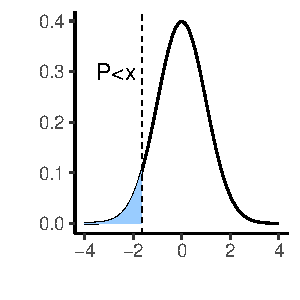
\includegraphics{Inferential-Stat-and-Z-test_files/figure-beamer/unnamed-chunk-1-1.pdf}

\centering

\tiny

\begin{itemize}
\tightlist
\item
  Decrease
\item
  Cooler
\item
  Smaller
\item
  Lower\\
\end{itemize}

\hfill\break
\end{column}

\begin{column}{0.5\textwidth}
\vspace{1cm}

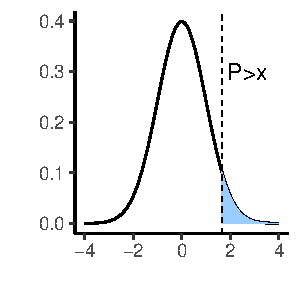
\includegraphics{Inferential-Stat-and-Z-test_files/figure-beamer/unnamed-chunk-2-1.pdf}

\centering

\tiny

\begin{itemize}
\tightlist
\item
  Increase
\item
  Warmer
\item
  Higher
\item
  Expand\\
\end{itemize}

\hfill\break
\end{column}
\end{columns}
\end{frame}

\begin{frame}{Expanding on Hypothesis Testing}
\phantomsection\label{expanding-on-hypothesis-testing-1}
\begin{itemize}
\tightlist
\item
  1-tailed - hypothesis includes an \textbf{expected direction}.
\end{itemize}

\begin{columns}[T]
\begin{column}{0.5\textwidth}
\vspace{1cm}

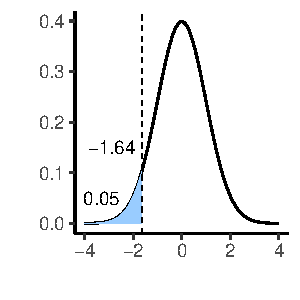
\includegraphics{Inferential-Stat-and-Z-test_files/figure-beamer/unnamed-chunk-3-1.pdf}
\end{column}

\begin{column}{0.5\textwidth}
\vspace{1cm}

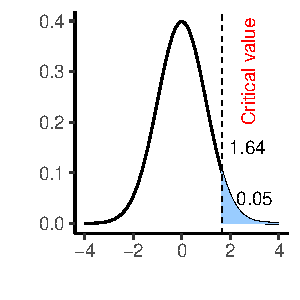
\includegraphics{Inferential-Stat-and-Z-test_files/figure-beamer/unnamed-chunk-4-1.pdf}
\end{column}
\end{columns}

\begin{itemize}
\tightlist
\item
  If your obtained test statistic falls beyond the critical value
  (lightblue) for your given Alpha threshold = Significant result,
  \textbf{reject the null}.
\end{itemize}
\end{frame}

\begin{frame}{Expanding on Hypothesis Testing}
\phantomsection\label{expanding-on-hypothesis-testing-2}
\begin{itemize}
\tightlist
\item
  2-tailed tests:

  \begin{itemize}
  \tightlist
  \item
    Have \textbf{no expected directionality} hypothesized.
  \item
    Splits the 5\% of the area under the curve that would be considered
    significant between both tails of the normal distribution curve.
  \item
    Are therefore less powerful tests (more likely to find a significant
    result).
  \end{itemize}
\end{itemize}

\centering

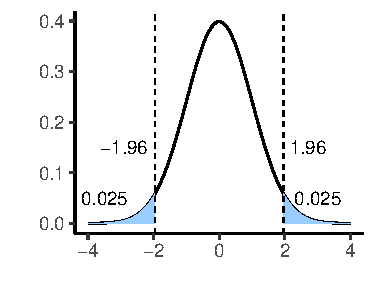
\includegraphics{Inferential-Stat-and-Z-test_files/figure-beamer/unnamed-chunk-5-1.pdf}\\
\end{frame}

\begin{frame}{Significant or Not?}
\phantomsection\label{significant-or-not}
\begin{columns}[T]
\begin{column}{0.5\textwidth}
\begin{itemize}
\item
  \textbf{Not significant}: \vspace{1cm}
\item
  Accept the null hypothesis.
\end{itemize}

\begin{itemize}
\tightlist
\item
  There is \textbf{no} difference between the sample and population
  mean.
\end{itemize}

\begin{itemize}
\tightlist
\item
  Obtained test statistic \textless{} critical value threshold.
\end{itemize}

\begin{itemize}
\tightlist
\item
  p-value \textgreater{} alpha threshold (usually 0.05).
\end{itemize}
\end{column}

\begin{column}{0.5\textwidth}
\textbf{Significant}: \vspace{1cm}

\begin{itemize}
\tightlist
\item
  Reject the null hypothesis,
\end{itemize}

\begin{itemize}
\tightlist
\item
  There \textbf{is} a difference between the sample and population mean.
\end{itemize}

\begin{itemize}
\tightlist
\item
  Obtained test statistic \textgreater{} critical value threshold.
\end{itemize}

\begin{itemize}
\tightlist
\item
  p-value \textless{} alpha threshold (usually 0.05).
\end{itemize}
\end{column}
\end{columns}
\end{frame}

\begin{frame}{Basic steps for an \textbf{Inferential Test}}
\phantomsection\label{basic-steps-for-an-inferential-test}
\begin{columns}[T]
\begin{column}{0.7\textwidth}
\begin{itemize}
\tightlist
\item
  A statement of null hypothesis.
\end{itemize}

\begin{itemize}
\tightlist
\item
  Choose the appropriate test.
\end{itemize}

\begin{itemize}
\tightlist
\item
  Set the level of Type I error risk (alpha)
\end{itemize}

\begin{itemize}
\tightlist
\item
  Analyze data distribution
\end{itemize}

\begin{itemize}
\item
  Compute the test statistic (obtained) value
\item
  Assess significance:

  \begin{itemize}
  \tightlist
  \item
    Determine the critical value needed to reject the null hypothesis
    and compare it to your - calculated test statistic
  \item
    Determine the p-value associated with your calculated test statistic
  \end{itemize}
\end{itemize}

\begin{itemize}
\tightlist
\item
  Summarize
\end{itemize}
\end{column}

\begin{column}{0.3\textwidth}
contents\ldots{}
\end{column}
\end{columns}
\end{frame}

\begin{frame}{Basic steps for an \textbf{Inferential Test}}
\phantomsection\label{basic-steps-for-an-inferential-test-1}
\begin{itemize}
\item
  We can select an appropriate test simply by answering some questions.
\item
  What type of data do we have?

  \begin{itemize}
  \tightlist
  \item
    If we have \textbf{frequency data}, we select the Chi-square family.
  \item
    \textbf{Continuous and categorical variables} will have a variety of
    different tests depending on the research question:
  \end{itemize}
\item
  What type of research question are we considering?

  \begin{itemize}
  \tightlist
  \item
    If \textbf{comparing one sample mean} to a \textbf{population} =
    \textcolor{red}{z-test}.
  \item
    If focus is on \textbf{differences} we go to the family of tests
    concerned with comparing groups or treatments
    (i.e.~\textcolor{red}{t-tests, ANOVA}).
  \item
    If the focus is on \textbf{relationships} between variables, we go
    to the \textcolor{red}{correlation tests}.
  \item
    If we want to \textbf{predict outcomes} we go to the
    \textcolor{red}{regression family}.
  \end{itemize}
\end{itemize}

\begin{columns}[T]
\begin{column}{0.4\textwidth}
\centering

\(y = \beta_0 + \beta_1 x + \epsilon\)
\end{column}

\begin{column}{0.6\textwidth}
where:\\
- \(y\) is the dependent variable,\\
- \(x\) is the independent variable,\\
- \(\beta_0\) is the intercept,\\
- \(\beta_1\) is the slope,\\
- \(\epsilon\) is the error term.
\end{column}
\end{columns}
\end{frame}

\begin{frame}{Basic steps for an \textbf{Inferential Test}}
\phantomsection\label{basic-steps-for-an-inferential-test-2}
\begin{itemize}
\item
  We can select an appropriate test simply by answering some questions.

  \begin{itemize}
  \item
    How many variables, how many groups are we including? (multivariate)
  \item
    Are observations independent from each other or purposely paired?
  \item
    Is my data not normally distributed? (non-parametric tests)
  \end{itemize}
\end{itemize}
\end{frame}

\begin{frame}{Statistical shorthand \textbf{z-test} example}
\phantomsection\label{statistical-shorthand-z-test-example}
\centering

\(z_{100} = 1.4, p = 0.16\)\\
\end{frame}

\begin{frame}{Statistical shorthand \textbf{z-test} example}
\phantomsection\label{statistical-shorthand-z-test-example-1}
\centering

\(z_{100} = 1.4, \, p = 0.16\) \[
\text{\huge $\downarrow$} \quad
\] \centering \[
\underbrace{z_{\underbrace{100}_{\text{Sample size}}}}_{\text{Test statistic}} = \underbrace{1.4}_{\text{z-value}}, \quad \underbrace{p = 0.16}_{\text{p-value}}
\]

\begin{itemize}
\tightlist
\item
  Every statistical test has a letter designating the type of test.
\item
  Because power is so closely tied to sample size, we report sample
  size.
\item
  For clarity (and to confirm the correct-tailed test is used to assess
  the p-value), include the calculated test statistic value.
\item
  Always report the p-value.
\item
  Some tests will also include a secondary metric to assess how
  meaningful results are (if significant).
\end{itemize}
\end{frame}

\begin{frame}{How to summarize your analysis: Key Components of a
Statistical Summary}
\phantomsection\label{how-to-summarize-your-analysis-key-components-of-a-statistical-summary}
\textcolor{teal}{Before installing a new air quality monitoring instrument, we tested to see if a sample of measurements taken at the testing lab differed significantly different from the long-term mean for the larger network population.}

\textcolor{orange}{Using a 2-tailed, one-sample z-test for on our normally distributed samples (W = 0.78).}

\textcolor{blue}{While the mean of the new instrument sample was slightly higher (sample mean = 117 vs. population mean = 108), we found no significant difference (z(100) = 1.4, p = 0.16).}

\textcolor{darkgray}{Based on these results we approve the installation of this instrument at the new site. However, we would suggest statistical comparisons of the current and new unit side-by-side, prior to decommissioning the current instrument.}
\end{frame}

\begin{frame}{How to summarize your analysis: Key Components of a
Statistical Summary}
\phantomsection\label{how-to-summarize-your-analysis-key-components-of-a-statistical-summary-1}
\textcolor{teal}{Introduction/Background:\\
Before installing a new air quality monitoring instrument, we tested to see if a sample of measurements taken at the testing lab differed significantly different from the long-term mean for the larger network population.}

\textcolor{orange}{Methods:\\
Using a 2-tailed, one-sample z-test for on our normally distributed samples (W = 0.78).}

\textcolor{blue}{Results:\\
While the mean of the new instrument sample was slightly higher (sample mean = 117 vs. population mean = 108), we found no significant difference \( z_{100} = 1.4, \, p = 0.16 \).}

\textcolor{darkgray}{Implications:\\
Based on these results we approve the installation of this instrument at the new site. However, we would suggest statistical comparisons of the current and new unit side-by-side, prior to decommissioning the current instrument.}
\end{frame}

\begin{frame}{}
\phantomsection\label{section}
\vspace{2cm}
\centering

\textcolor{blue}{Our First Inferential Tests!\\
One sample z-test}\\
\strut \\
\strut \\
\end{frame}

\begin{frame}{When would you run a one-sample z-test?}
\phantomsection\label{when-would-you-run-a-one-sample-z-test}
\begin{itemize}
\tightlist
\item
  Use the One Sample z-test when:

  \begin{itemize}
  \tightlist
  \item
    You want to test for a difference between one sample mean and a
    larger population mean.
  \item
    There is only one group (sample) being tested against the larger
    population.
  \item
    You know (or can estimate) the mean and standard deviation of the
    population.
  \item
    Data is normally distributed.
  \end{itemize}
\end{itemize}

\[
z = \frac{\bar{X} - \mu}{\frac{\sigma}{\sqrt{n}}}
\]

where:\\
- \(\bar{X}\): Sample mean.\\
- \(\mu\): Population mean.\\
- \(\sigma\): Population standard deviation. - \(n\): Sample size.
\end{frame}

\begin{frame}{When would you run a one-sample z-test?}
\phantomsection\label{when-would-you-run-a-one-sample-z-test-1}
\begin{itemize}
\tightlist
\item
  Use the One Sample z-test when:

  \begin{itemize}
  \tightlist
  \item
    You want to test for a difference between one sample mean and a
    larger population mean.
  \item
    There is only one group (sample) being tested against the larger
    population.
  \item
    You know (or can estimate) the mean and standard deviation of the
    population.

    \begin{itemize}
    \tightlist
    \item
      \textcolor{orange}{Expert Information.}
    \item
      \textcolor{orange}{Scientific Literature.}
    \item
      \textcolor{orange}{Data archives.}
    \item
      \textcolor{orange}{Meaningful (hypothesized value).}
    \end{itemize}
  \item
    Data is normally distributed.
  \end{itemize}
\end{itemize}
\end{frame}

\begin{frame}{Flowcharts: Keeping it simple with questions}
\phantomsection\label{flowcharts-keeping-it-simple-with-questions}
\end{frame}

\begin{frame}{One sample z-test}
\phantomsection\label{one-sample-z-test}
Assume you have a sample of \textbf{20 observations}. The mean of this
\textbf{sample is 150}, and you want to determine whether there is a
\textbf{difference between the sample mean and the larger population
mean}. Since you are not specifying a direction for this difference, you
will conduct a two-tailed test.

The \textbf{population mean is 164}, and the \textbf{population standard
deviation is 33}.

Next, calculate the obtained value for this \textbf{one-sample z-test.}

\begin{columns}[T]
\begin{column}{0.5\textwidth}
\vspace{1cm}

\[
z = \frac{\bar{X} - \mu}{\frac{\sigma}{\sqrt{n}}}
\]
\end{column}

\begin{column}{0.5\textwidth}
\vspace{1cm}

\[
z = \frac{150 - 164}{\frac{33}{\sqrt{20}}} = -1.897
\]
\end{column}
\end{columns}
\end{frame}

\begin{frame}{One sample z-test}
\phantomsection\label{one-sample-z-test-1}
Assume you have a sample of \textbf{20 observations}. The mean of this
\textbf{sample is 150}, and you want to determine whether there is a
\textbf{difference between the sample mean and the larger population
mean}. Since you are not specifying a direction for this difference, you
will conduct a two-tailed test.

The \textbf{population mean is 164}, and the \textbf{population standard
deviation is 33}.

Next, calculate the obtained value for this \textbf{one-sample z-test.}

\begin{columns}[T]
\begin{column}{0.5\textwidth}
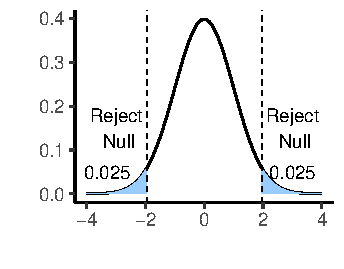
\includegraphics{Inferential-Stat-and-Z-test_files/figure-beamer/unnamed-chunk-6-1.pdf}
\end{column}

\begin{column}{0.5\textwidth}
\vspace{1cm}

\[
z = \frac{150 - 164}{\frac{33}{\sqrt{20}}} = -1.897
\]
\end{column}
\end{columns}
\end{frame}

\begin{frame}{Critical Value Approach}
\phantomsection\label{critical-value-approach}
\begin{itemize}
\tightlist
\item
  In the critical value approach, we compare the calculated test
  statistic to the critical value from the standard normal distribution.
  For a two-tailed test at the \(\alpha = 0.05\) significance level, the
  critical values are approximately ±1.96, which corresponds to the
  \textbf{0.025} in each tail.
\end{itemize}

\vspace{1cm}

\begin{itemize}
\item
  Decision Rule
\item
  If \(| \text{calculated test statistic} | > \text{critical value}\) =
  \textbf{Significant}
\item
  If \(| \text{calculated test statistic} | \leq \text{critical value}\)
  = \textbf{Not Significant}
\end{itemize}
\end{frame}

\begin{frame}{Critical Value Approach}
\phantomsection\label{critical-value-approach-1}
In this case:

\centering

\[
|-1.897| < 1.96
\]\\

\begin{itemize}
\tightlist
\item
  Thus, we fail to reject the null hypothesis, indicating that there is
  \textbf{no significant} difference between the sample mean and the
  population mean.
\end{itemize}
\end{frame}

\begin{frame}[fragile]{Finding the p-value}
\phantomsection\label{finding-the-p-value}
Now we need to determine the probability (p-value) associated with the
calculated test statistic. You have several options to achieve this:

\begin{Shaded}
\begin{Highlighting}[]
\NormalTok{z\_value }\OtherTok{\textless{}{-}} \SpecialCharTok{{-}}\FloatTok{1.897}
\NormalTok{p\_value }\OtherTok{\textless{}{-}} \DecValTok{2} \SpecialCharTok{*} \FunctionTok{pnorm}\NormalTok{(z\_value)  }\CommentTok{\# Two{-}tailed p{-}value}
\NormalTok{p\_value  }\CommentTok{\# This will give the result}
\end{Highlighting}
\end{Shaded}

\begin{verbatim}
## [1] 0.05782794
\end{verbatim}

\begin{itemize}
\tightlist
\item
  Since this p-value (0.0578) is greater than the alpha threshold of
  0.05, we conclude that the result is \textbf{not significant}.
\end{itemize}
\end{frame}

\begin{frame}{Example: Car rental}
\phantomsection\label{example-car-rental}
\end{frame}

\begin{frame}{Example: Car rental}
\phantomsection\label{example-car-rental-1}
\begin{itemize}
\item
  A rental car company claims the mean time to rent a car on their
  \textbf{website is 60 seconds with a standard deviation of 30
  seconds}. A random sample \textbf{36 customers} attempted to rent a
  car on the website. The \textbf{mean time to rent was 75 seconds}. Is
  this enough evidence to contradict the company's claim? \vspace{0.5cm}
\item
  Step 1: Set up the hypotheses \vspace{0.5cm}
\end{itemize}

\begin{columns}[T]
\begin{column}{0.5\textwidth}
\begin{itemize}
\tightlist
\item
  \textbf{Null hypothesis (\(H_0\))}: The mean rental time is 60
  seconds. \[
  H_0: \mu = 60
  \]
\end{itemize}
\end{column}

\begin{column}{0.5\textwidth}
\begin{itemize}
\tightlist
\item
  \textbf{Alternative hypothesis (\(H_1\))}: The mean rental time is
  greater than 60 seconds. \[
  H_1: \mu > 60
  \]
\end{itemize}
\end{column}
\end{columns}
\end{frame}

\begin{frame}{Example: Car rental}
\phantomsection\label{example-car-rental-2}
\begin{itemize}
\item
  A rental car company claims the mean time to rent a car on their
  \textbf{website is 60 seconds with a standard deviation of 30
  seconds}. A random sample \textbf{36 customers} attempted to rent a
  car on the website. The \textbf{mean time to rent was 75 seconds}. Is
  this enough evidence to contradict the company's claim? \vspace{0.5cm}
\item
  Step 2: Test statistic formula \vspace{0.5cm}
\end{itemize}

\begin{columns}[T]
\begin{column}{0.5\textwidth}
\[
z = \frac{\bar{X} - \mu}{\frac{\sigma}{\sqrt{n}}}
\]
\end{column}

\begin{column}{0.5\textwidth}
\[
z = \frac{75 - 60}{\frac{30}{\sqrt{36}}} = \frac{15}{5} = 3
\]
\end{column}
\end{columns}
\end{frame}

\begin{frame}[fragile]{Example: Car rental}
\phantomsection\label{example-car-rental-3}
\begin{itemize}
\item
  A rental car company claims the mean time to rent a car on their
  \textbf{website is 60 seconds with a standard deviation of 30
  seconds}. A random sample \textbf{36 customers} attempted to rent a
  car on the website. The \textbf{mean time to rent was 75 seconds}. Is
  this enough evidence to contradict the company's claim? \vspace{0.5cm}
\item
  Step 3: Set up the hypotheses
\end{itemize}

\begin{columns}[T]
\begin{column}{0.4\textwidth}
For a \textbf{one-tailed test} at a significance level of
\(\alpha = 0.05\), the critical z-value is approximately \textbf{1.645}
(since we are only looking at one tail).
\end{column}

\begin{column}{0.6\textwidth}
\begin{Shaded}
\begin{Highlighting}[]
\CommentTok{\# Given z{-}value}
\NormalTok{z\_value }\OtherTok{\textless{}{-}} \DecValTok{3}
\CommentTok{\# Calculate the one{-}tailed p{-}value}
\NormalTok{p\_value }\OtherTok{\textless{}{-}} \DecValTok{1} \SpecialCharTok{{-}} \FunctionTok{pnorm}\NormalTok{(z\_value)}
\CommentTok{\# Print the p{-}value}
\NormalTok{p\_value}
\end{Highlighting}
\end{Shaded}

\begin{verbatim}
## [1] 0.001349898
\end{verbatim}
\end{column}
\end{columns}
\end{frame}

\begin{frame}{Example: Car rental}
\phantomsection\label{example-car-rental-4}
\textcolor{teal}{We tested a rental car company's claim that reservations could be made online in 60 seconds on average.}
\textcolor{orange}{ Using a random sample of 36 online rentals in a one-tailed, one-sample z-test}
\textcolor{blue}{ we found that mean reservation time is actually significantly higher than the company claims (\( z_{(36)}=3, \, p=0.001 \)).}
\textcolor{darkgray}{  This result indicates that it is highly unlikely customers can rent a car in 60 seconds as claimed.  We suggest that the rental company adjust its claim to match the 75 second mean encountered for our test sample to avoid misleading potential customers.}
\end{frame}

\end{document}
